% -------------------------------------------------------------------------------------------------------
%-----------------------------CONSULTA DE PLANES DE ESTUDIO Jefe de Departamento de Desarrollo e Innovación Curricular ---------------------------------
% -------------------------------------------------------------------------------------------------------

\section{Gestión de Plan de Estudios}
\subsection{Consulta de Planes de Estudios}
Cuando el Jefe de Departamento de Desarrollo e Innovación Curricular da clic a un programa académico en la sección de \textbf{Gestionar Programas Académicos} aparece la siguiente pantalla: 

% Imagen menu

\begin{figure}[!hbtp]
	\centering
	\hypertarget{consultarPE}{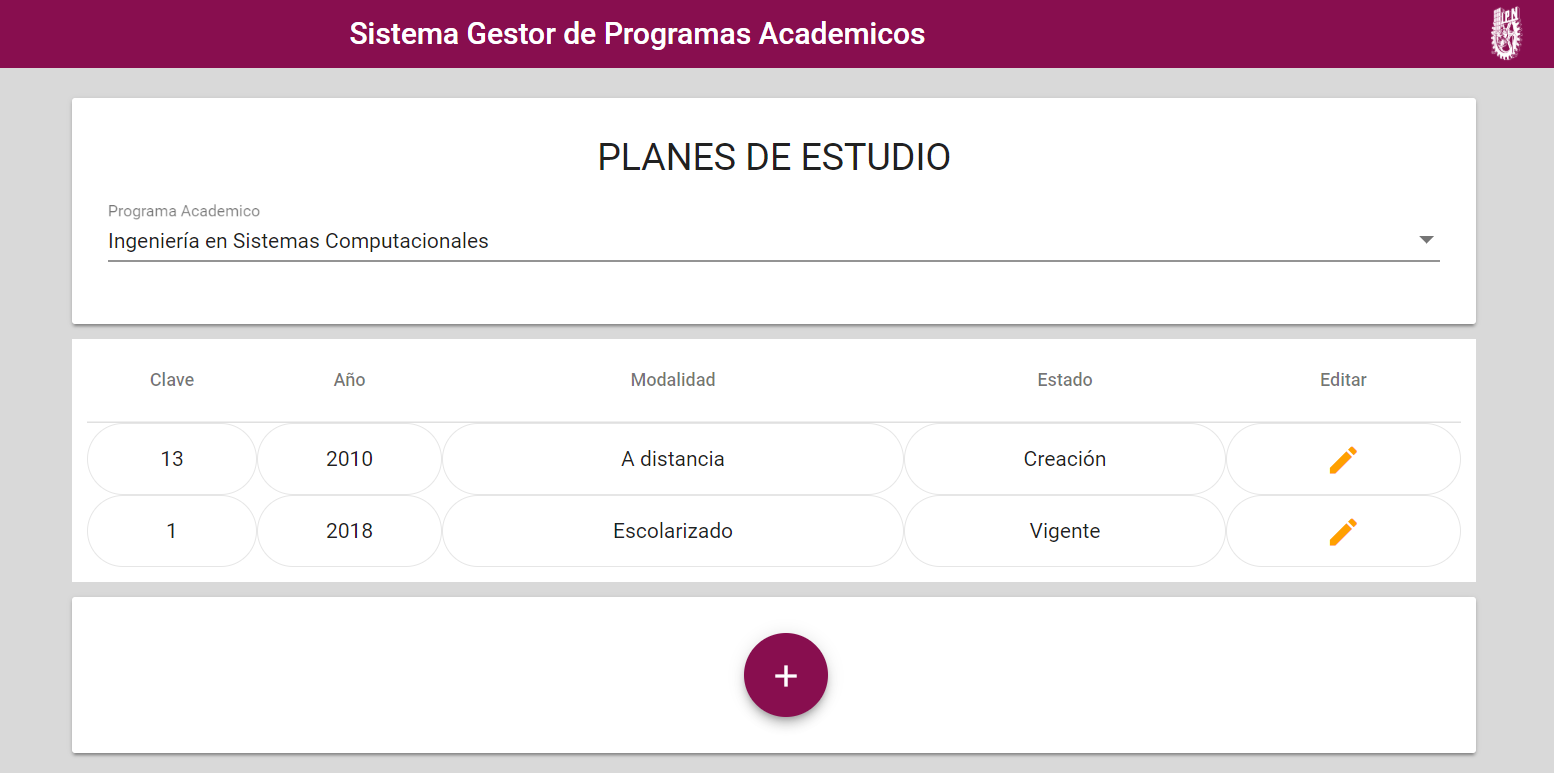
\includegraphics[width=0.7\linewidth]{images/SP4-GPE/consultar}}
	\caption{Pantalla para Planes de Estudio}
	\label{consultarPE}
\end{figure}

En donde se muestra un listado de todos los Planes de Estudios a su cargo. El Jefe de Departamento de Desarrollo e Innovación Curricular tiene a su disposición tres funciones:

\subsubsection{Buscar Planes de Estudio según el programa académico}

Para ello, el Jefe de Departamento de Desarrollo e Innovación Curricular tiene que seleccionar el Programa Académico que desea consultar en el siguiente componente:

\begin{figure}[!hbtp]
	\centering
	\hypertarget{academico}{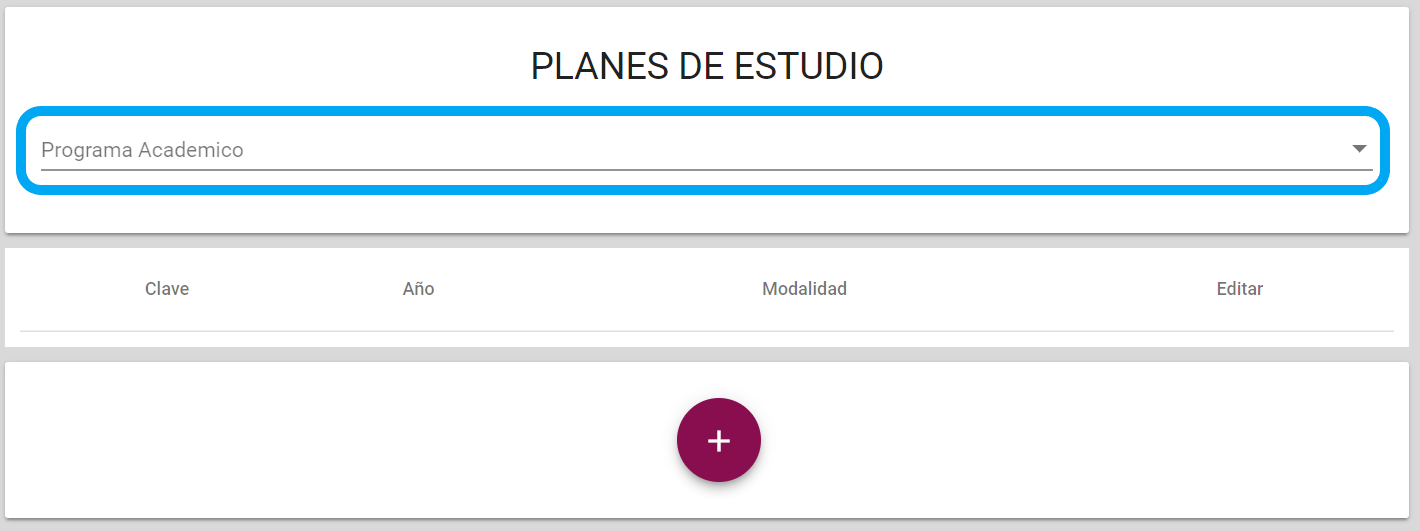
\includegraphics[width=0.7\linewidth]{images/SP4-GPE/programa}}
	\caption{Selección de Programa Académico}
	\label{academico}
\end{figure}

\begin{figure}[!hbtp]
	\centering
	\hypertarget{academico2}{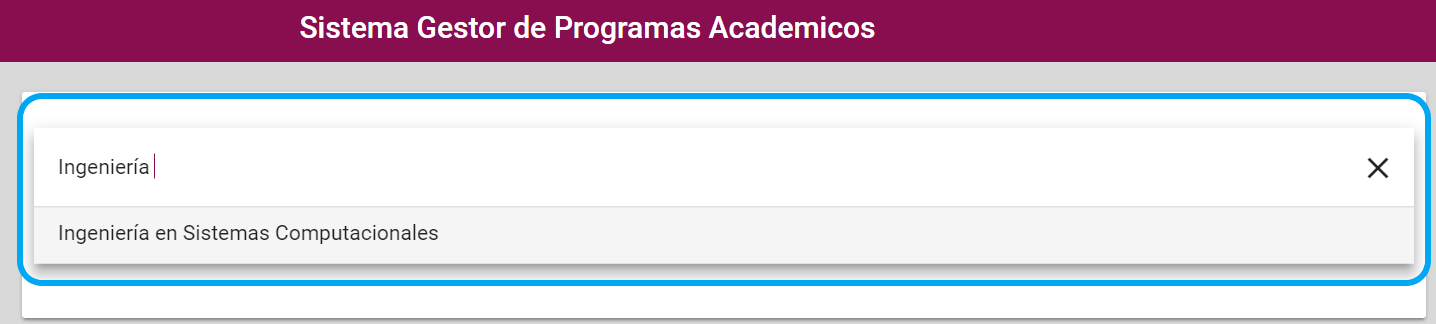
\includegraphics[width=0.7\linewidth]{images/SP4-GPE/programaD}}
	\caption{Despliegue de Programas Académicos}
	\label{academico2}
\end{figure}

A continuación el sistema muestra todos los Planes de Estudios que tengan el Programa Académico seleccionado.
\begin{figure}[!hbtp]
	\centering
	\hypertarget{planes}{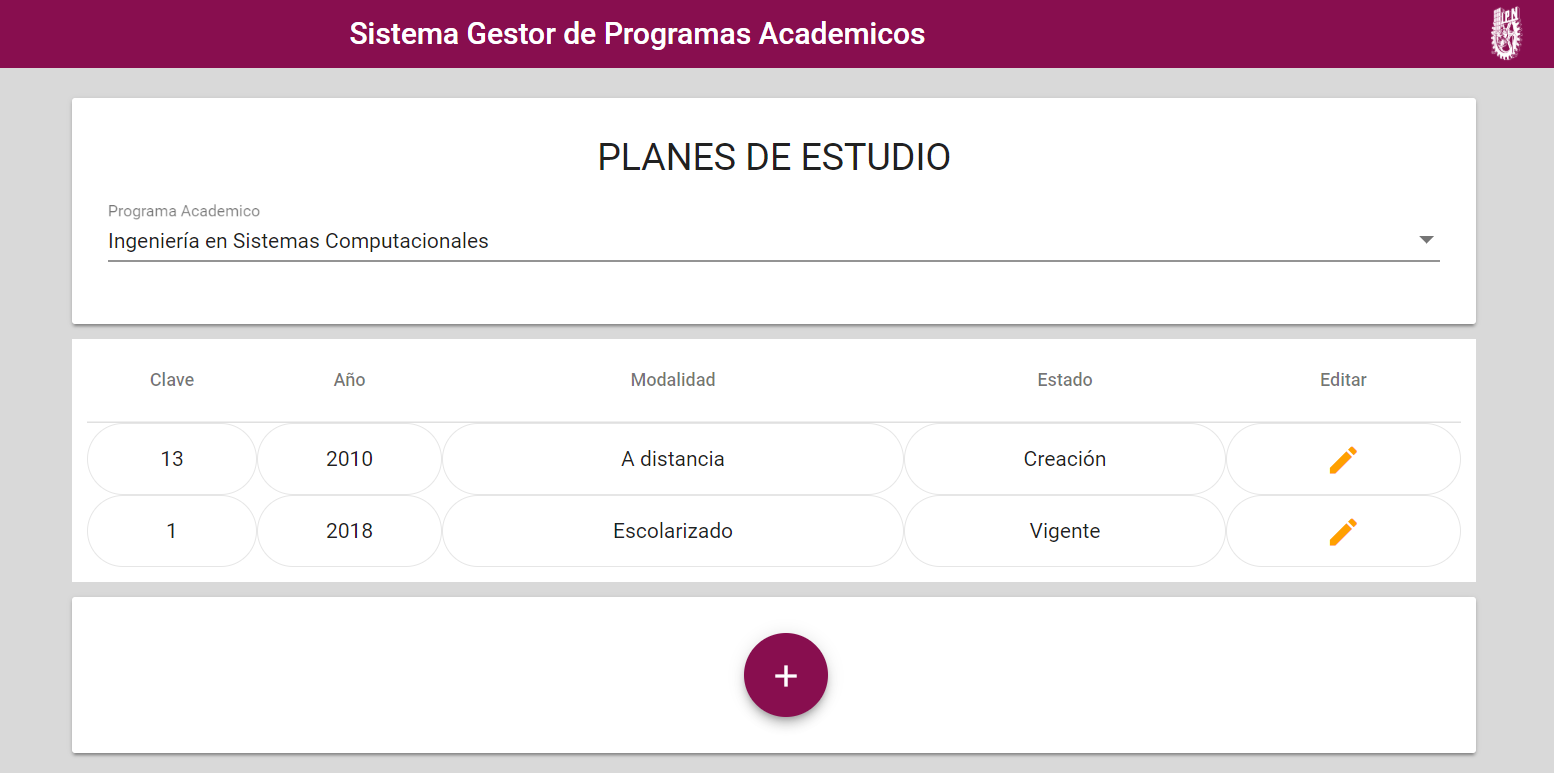
\includegraphics[width=0.7\linewidth]{images/SP4-GPE/consultar}}
	\caption{Planes de Estudios Encontrados}
	\label{planes}
\end{figure}
\newpage
\subsection{Editar Planes de Estudios}

Para ello, el Jefe de Departamento de Desarrollo e Innovación Curricular tiene que dar clic en el botón \IUbutton{Lápiz} que esta al lado del Plan de Estudio que desea modificar. Al hacer esto, el sistema redirecciona al usuario a la pantalla de \hyperlink{editarPE}{\textit{Editar Plan de Estudio}}.

\begin{figure}[!hbtp]
	\centering
	\hypertarget{editar}{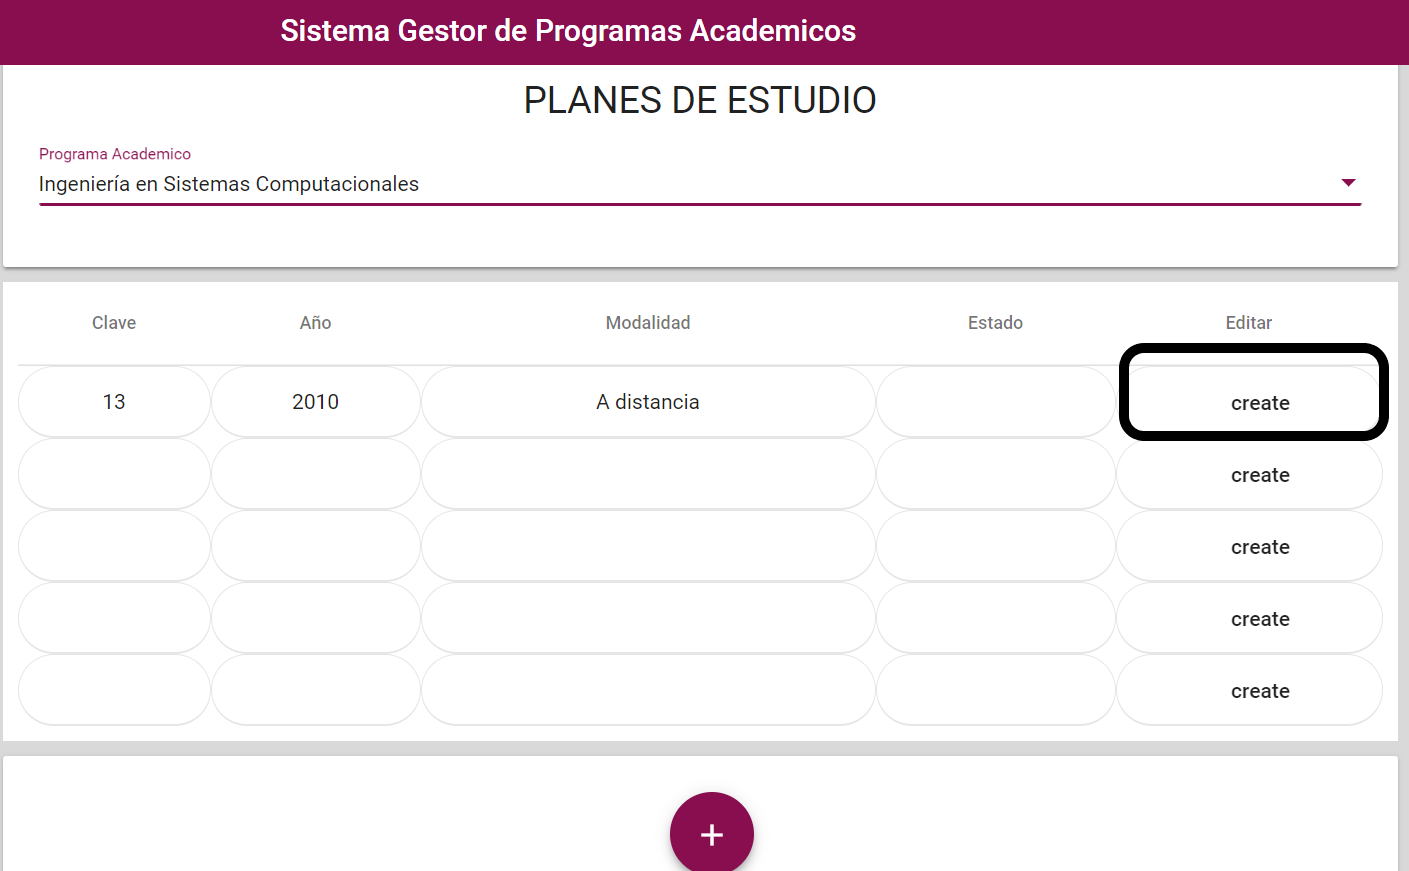
\includegraphics[width=0.7\linewidth]{images/SP4-GPE/editarC}}
	\caption{Botón Editar Plan de Estudio}
	\label{editar}
\end{figure}

\begin{figure}[!hbtp]
	\centering
	\hypertarget{editarPE}{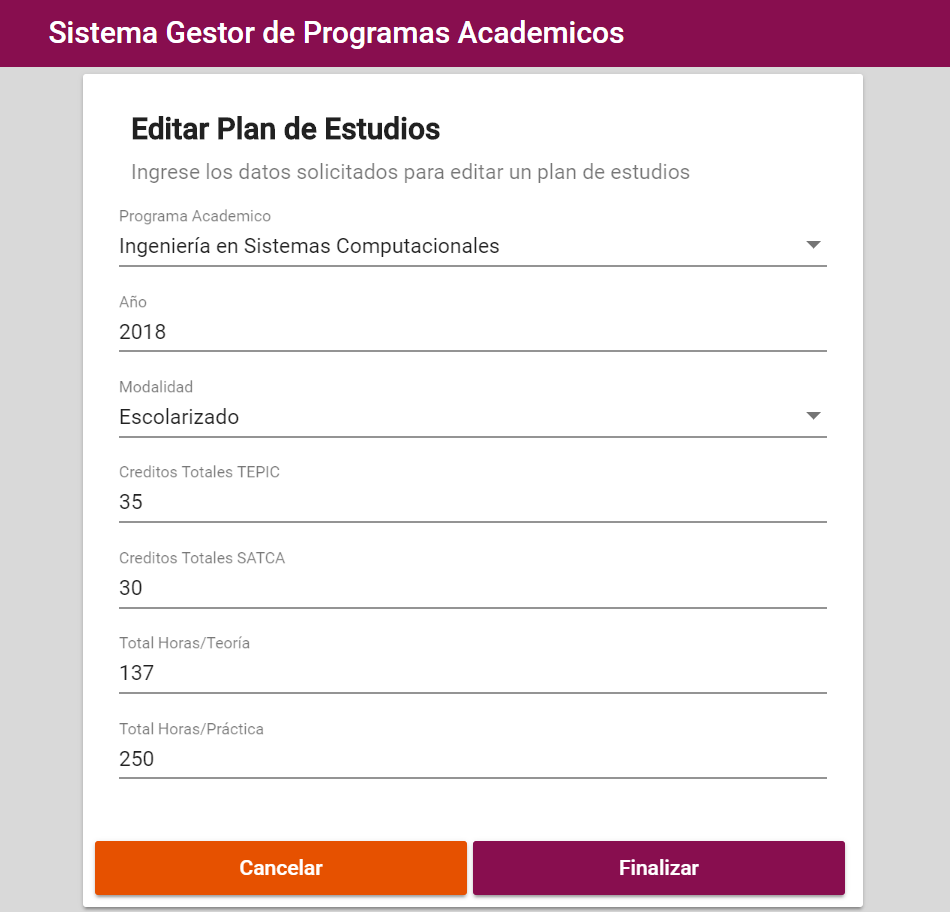
\includegraphics[width=0.7\linewidth]{images/SP4-GPE/editarPE}}
	\caption{Pantalla para la edición de Planes de Estudios}
	\label{editarPE}
\end{figure}

En donde se cargan los datos del Plan de Estudio seleccionado en la pantalla de \hyperlink{consultarPE}{\textit{Consultar Planes de Estudios}} y llena el formulario.
\newpage
A continuación, el Jefe de Departamento de Desarrollo e Innovación Curricular puede modificar todos los campos del Plan de Estudio.
\begin{figure}[!hbtp]
	\centering
	\hypertarget{modif}{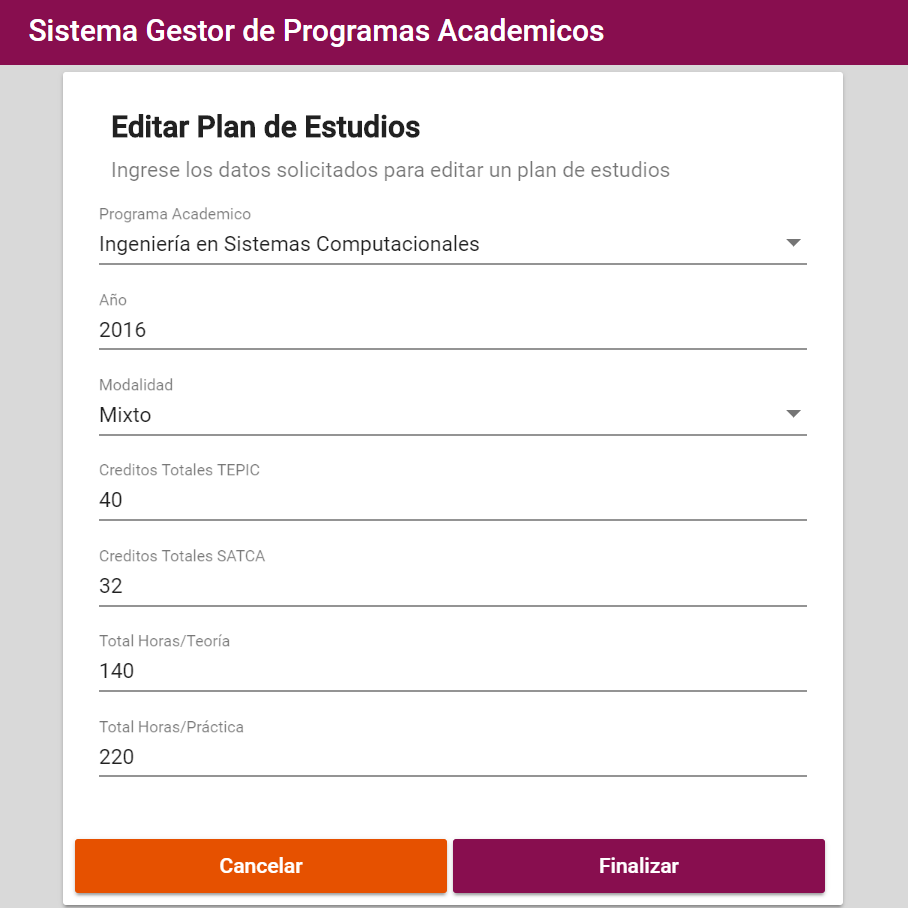
\includegraphics[width=0.7\linewidth]{images/SP4-GPE/editarPE1}}
	\caption{Datos del Plan de Estudio modificados}
	\label{modif}
\end{figure}

 Si el Jefe de Departamento de Desarrollo e Innovación Curricular da clic en el botón \IUbutton{Cancelar} sin haber concluido la edición del Plan de Estudio:

\begin{figure}[!hbtp]
	\centering
	\hypertarget{cancel2}{
\includegraphics[width=0.7\linewidth]{images/SP4-GPE/cancelarPE}}
	\caption{Botón ''Cancelar''}
	\label{cancel2}
\end{figure}
\newpage

El sistema mostrará el siguiente mensaje:
\begin{figure}[!hbtp]
	\centering
	\hypertarget{ms1}{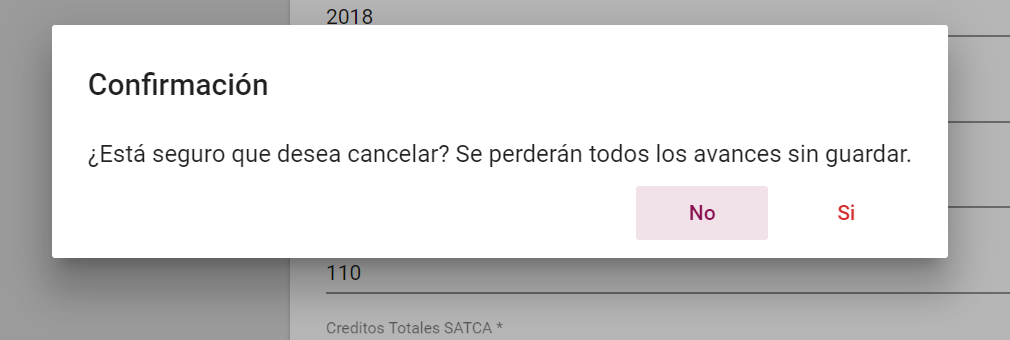
\includegraphics[width=0.7\linewidth]{images/SP4-GPE/m1}}
	\caption{Mensaje de cancelar}
	\label{ms1}
\end{figure}

Para confirmar, el Jefe de Departamento de Desarrollo e Innovación Curricular debe dar clic en el botón  \IUbutton{Si}, y el Plan de Estudio no es modificado.\\

Para cancelar, el Jefe de Departamento de Desarrollo e Innovación Curricular debe dar clic en botón  \IUbutton{No}, el mensaje se cierra y continuamos en el formulario. Aquí el Jefe de Departamento de Desarrollo e Innovación Curricular puede terminar la edición del Plan de Estudio.\\

Una vez que se modifican los datos,  el Jefe de Departamento de Desarrollo e Innovación Curricular debe de dar clic en el botón  \IUbutton{Finalizar}.
\begin{figure}[!hbtp]
	\centering
	\hypertarget{btnfin}{
\includegraphics[width=0.7\linewidth]{images/SP4-GPE/editarPER}}
	\caption{Botón ''Finalizar''}
	\label{btnfin}
\end{figure}

Si no exiten errores, el sistema muestra el siguiente mensaje:
%Imagen MSG27
\begin{figure}[!hbtp]
	\centering
	\hypertarget{ms2}{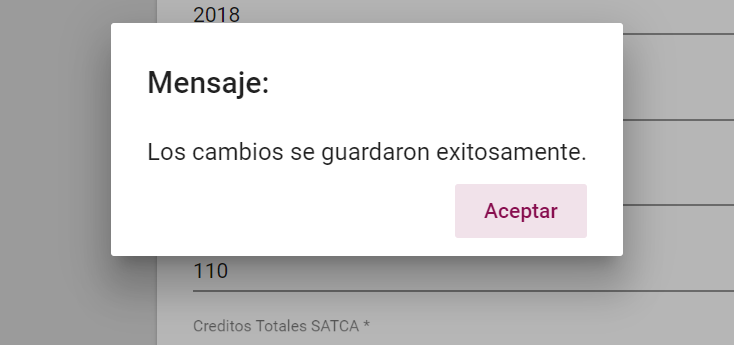
\includegraphics[width=0.7\linewidth]{images/SP4-GPE/m2}}
	\caption{Mensaje de modificar datos}
	\label{ms2}
\end{figure}


Al dar clic en en el botón  \IUbutton{Aceptar}, el sistema redirecciona al usuario a la pantalla de \hyperlink{consultarPE}{\textit{Consultar Planes de Estudios}}, en donde puede ver las modificaciones del Plan de Estudios.\\
\newpage
\subsubsection{Posibles errores}

\begin{itemize}
	\item Problemas con la conexión o el sistema

	Si el Jefe de Departamento de Desarrollo e Innovación Curricular accede a la pantalla de \hyperlink{editarPE}{\textit{Editar Plan de Estudio}} o intenta modificar un Plan de Estudio, aparece alguno de los siguientes mensajes:

	% Imagen MSG7 Y MSG25
	\begin{figure}[!hbtp]
		\centering
		\hypertarget{ms3}{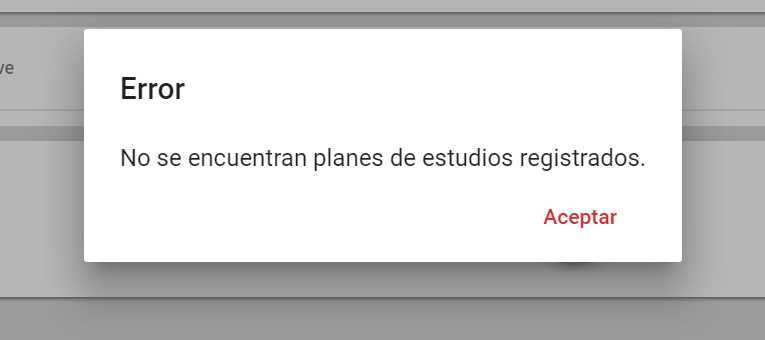
\includegraphics[width=0.7\linewidth]{images/SP4-GPE/m3}}
		\caption{Mensaje de ningun plan de estudios registrado}
		\label{ms3}
	\end{figure}
	\begin{figure}[!hbtp]
		\centering
		\hypertarget{error}{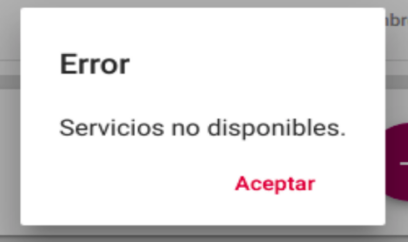
\includegraphics[width=0.7\linewidth]{images/SP4-GPE/error}}
		\caption{Servicios no disponibles}
		\label{error}
	\end{figure}


	Significa que hay un error de conexión. Al dar clic en en botón  \IUbutton{Aeptar}, el sistema redirecciona al Jefe de Departamento de Desarrollo e Innovación Curricular a la pantalla de \hyperlink{consultarPE}{\textit{Consultar Planes de Estudios}}. 
	\newpage

	\item Campos vacíos al momento de que se modifica el Plan de Estudio

	Si el Jefe de Departamento de Desarrollo e Innovación Curricular deja en blanco algún campo del formulario, y posteriormente da clic en el botón  \IUbutton{Registrar}, el sistema mostrará el siguiente mensaje:

	% Imagen MSG32
		\begin{figure}[!hbtp]
		\centering
		\hypertarget{ms4}{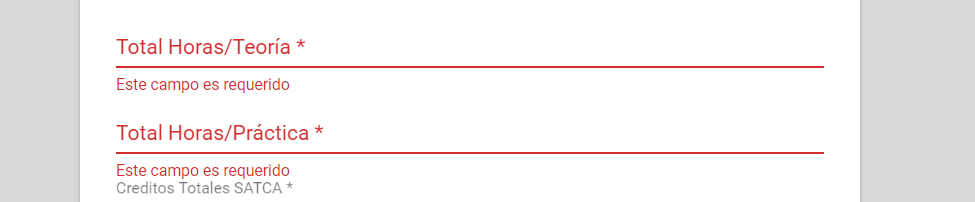
\includegraphics[width=0.7\linewidth]{images/SP4-GPE/m4}}
		\caption{Campo Obligatorio}
		\label{ms4}
	\end{figure}

	 El Jefe de Departamento de Desarrollo e Innovación Curricular debe llenar el o los campos que dejo vacíos. Si se continúan dejando campos en blanco y dando clic en el botón  \IUbutton{Registrar}, aparece nuevamente el mensaje, hasta que todos los campos son llenados.


	\item Los campos ingresados no son válidos

	Si al momento de dar clic en el \IUbutton{Registrar} aparece el siguiente mensaje:
	% Imagen MSG20
	\begin{figure}[!hbtp]
		\centering
		\hypertarget{ms5}{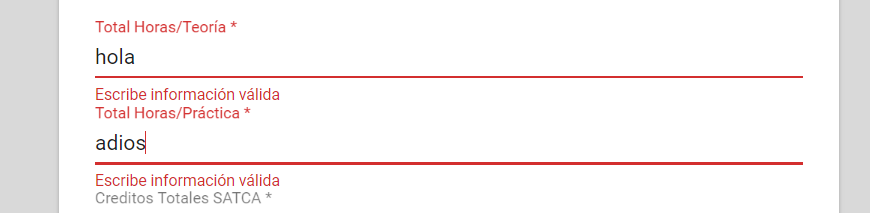
\includegraphics[width=0.7\linewidth]{images/SP4-GPE/m5}}
		\caption{Datos no válidos}
		\label{ms5}
	\end{figure}

	Significa que la composición de los datos ingresados en el formulario no es la correcta, verifíquelos e intente de nuevo.

\end{itemize}


\newpage
\subsection{Registrar Planes de Estudios}

Para ello, el Jefe de Departamento de Desarrollo e Innovación Curricular debe dar clic en el botón \IUbutton{+} en la parte inferior de la pantalla.

\begin{figure}[!hbtp]
	\centering
	\hypertarget{add}{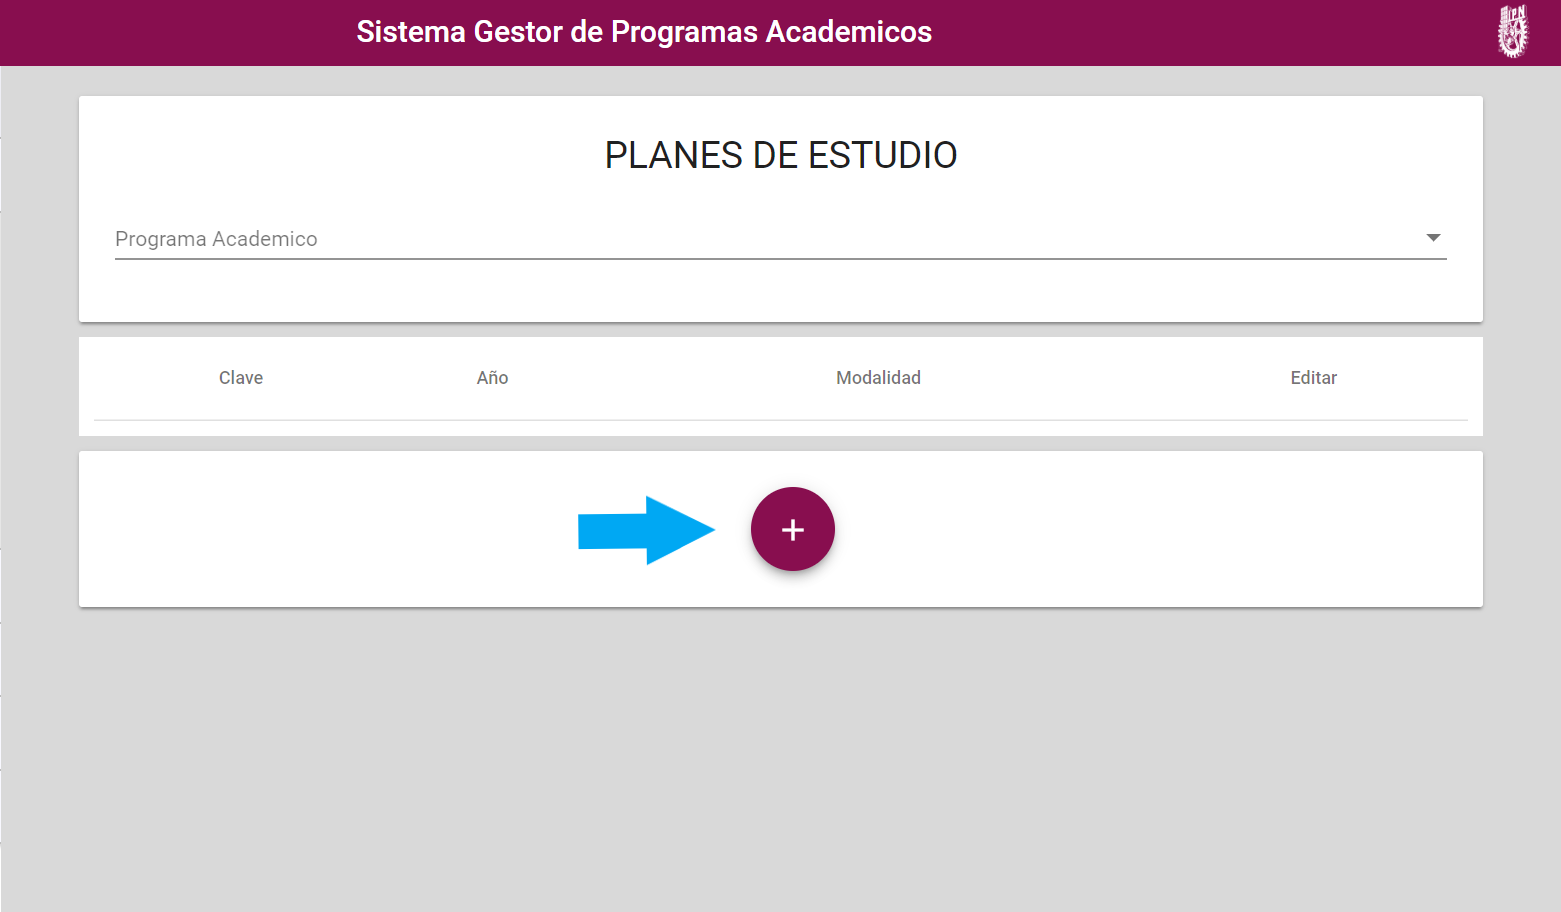
\includegraphics[width=0.7\linewidth]{images/SP4-GPE/mas}}
	\caption{Botón Agregar Plan de Estudio}
	\label{add}
\end{figure}

Al hacerlo, el sistema redirecciona al Jefe de Departamento de Desarrollo e Innovación Curricular a la pantalla de \hyperlink{registrarPE}{\textit{Registrar Plan de Estudio}}.


\textbf{NOTA:} En caso de que exista un error de conexión, aparecerá el siguiente mensaje:
%Imagen del MSG7
	\begin{figure}[!hbtp]
	\centering
	\hypertarget{error}{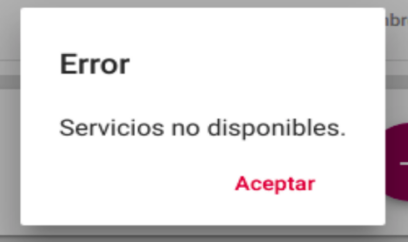
\includegraphics[width=0.7\linewidth]{images/SP4-GPE/error}}
	\caption{Servicios no disponibles}
	\label{error}
\end{figure}

Al dar clic en en botón \IUbutton{Aceptar}, el sistema redirecciona  al Jefe de Departamento de Desarrollo e Innovación Curricular a la pantalla de \hyperlink{registrarPE}{\textit{Registrar Plan de Estudio}}. 
\newpage
\subsubsection{Registro de Plan de Estudio}
Si el Jefe de Departamento de Desarrollo e Innovación Curricular en la pantalla de \hyperlink{consultarPE}{\textit{Consultar Planes de Estudios}} da clic en el botón \IUbutton{+}, aparece la siguiente pantalla:

\begin{figure}[!hbtp]
	\centering
	\hypertarget{registrarPE}{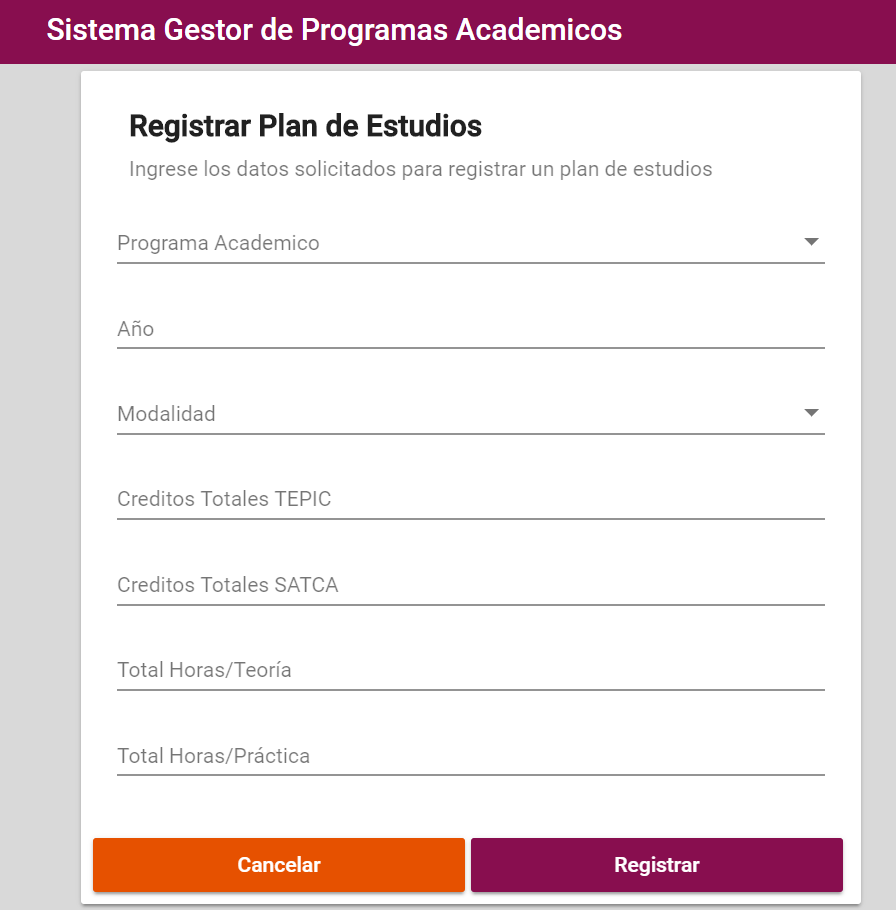
\includegraphics[width=0.7\linewidth]{images/SP4-GPE/registrarPE}}
	\caption{Pantalla para registrar Planes de Estudio}
	\label{registrarPE}
\end{figure}
\newpage
En donde tiene que ingresar los campos del nuevo Plan de Estudio o en el formulario. Un ejemplo del llenado es el siguiente:

\begin{figure}[!hbtp]
	\centering
	\hypertarget{ejreg}{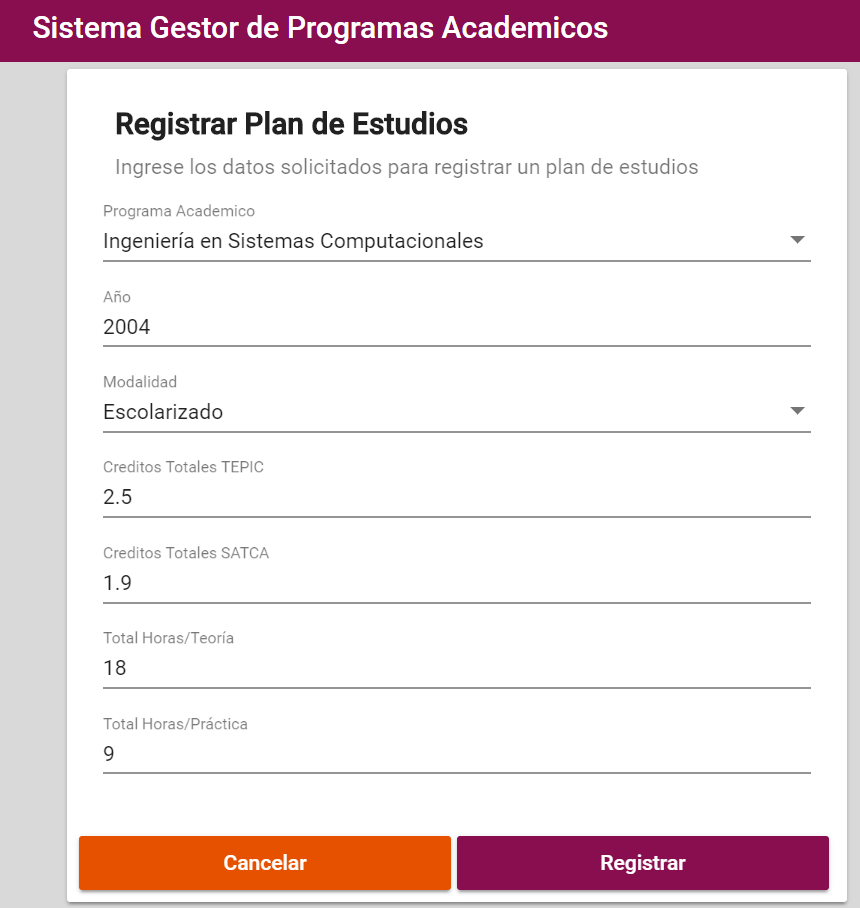
\includegraphics[width=0.7\linewidth]{images/SP4-GPE/registrarEjem}}
	\caption{Ejemplo de llenado para agregar un nuevo Plan de Estudios}
	\label{ejreg}
\end{figure}
%\newpage
Si el Jefe de Departamento de Desarrollo e Innovación Curricular da clic en el botón \IUbutton{Cancelar} sin haber concluido el registro del Plan de Estudio:

\begin{figure}[!hbtp]
	\centering
	\hypertarget{cancel2}{
\includegraphics[width=0.7\linewidth]{images/SP4-GPE/cancelarPE}}
	\caption{Botón Cancelar}
	\label{cancel2}
\end{figure}
\newpage

El sistema muestra el siguiente mensaje:
%Imagen MSG30
\begin{figure}[!hbtp]
	\centering
	\hypertarget{ms1}{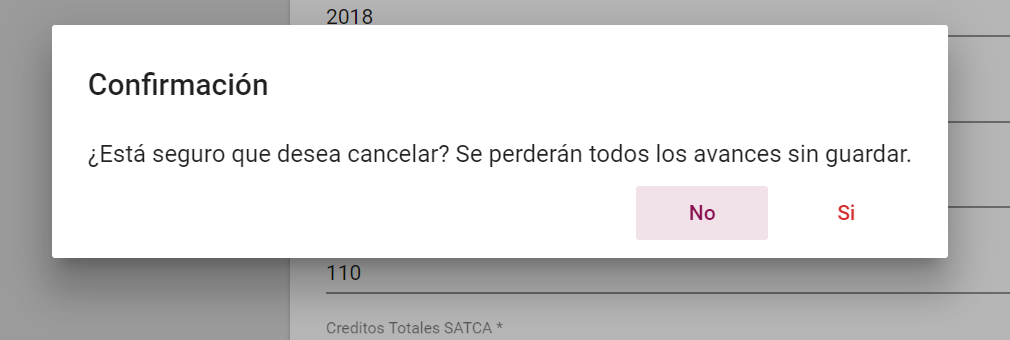
\includegraphics[width=0.7\linewidth]{images/SP4-GPE/m1}}
	\caption{Mensaje de cancelar}
	\label{ms1}
\end{figure}

Para confirmar,  el Jefe de Departamento de Desarrollo e Innovación Curricular da clic en el botón  \IUbutton{Si}, y el Plan de Estudio no es registrado.\\

Para cancelar, el Jefe de Departamento de Desarrollo e Innovación Curricular da clic en botón  \IUbutton{No}, el mensaje se cierra y continuamos en el formulario. Aquí el Jefe de Departamento de Desarrollo e Innovación Curricular puede terminar la edición del Plan de Estudio.

A continuación, una vez verificados los datos, debe de dar clic en el botón \IUbutton{Registrar}.
\begin{figure}[!hbtp]
	\centering
	\hypertarget{btnreg}{
\includegraphics[width=0.7\linewidth]{images/SP4-GPE/registrarB}}
	\caption{Botón Registrar}
	\label{btnreg}
\end{figure}

Si no existen errores, el sistema muestra el siguiente mensaje:
% Imagen MSG5
	\begin{figure}[!hbtp]
	\centering
	\hypertarget{exito}{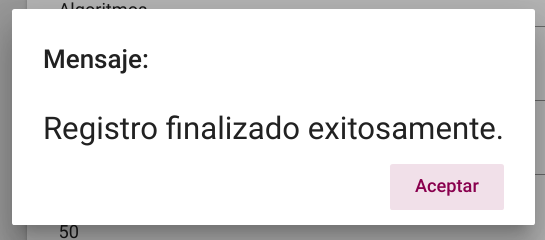
\includegraphics[width=0.7\linewidth]{images/SP4-GPE/exito}}
	\caption{Registro exitoso}
	\label{exito}
\end{figure}

Al dar clic en en botón \IUbutton{Aceptar}, el sistema redirecciona  al Jefe de Departamento de Desarrollo e Innovación Curricular a la pantalla de \hyperlink{consultarPE}{\textit{Consultar Planes de Estudios}}, en donde puede ver el nuevo Plan de Estudios agregado.\\
\newpage
\subsubsection{Posibles errores}
\begin{itemize}
	
	\item Problemas con la conexión o el sistema
	
	Si al momento de acceder a la pantalla de \hyperlink{registrarPE}{\textit{Registrar Plan de Estudios}}, aparece alguno de los siguientes mensajes:
	%Imagen MSG7 Y MSG25
		\begin{figure}[!hbtp]
		\centering
		\hypertarget{error}{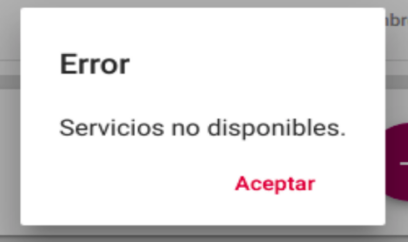
\includegraphics[width=0.7\linewidth]{images/SP4-GPE/error}}
		\caption{Servicios no disponibles}
		\label{error}
		\end{figure}
	
	
	Significa que existe un error de conexión o del sistema. Al dar clic en en botón \IUbutton{Aceptar}, el sistema redirecciona al Jefe de Departamento de Desarrollo e Innovación Curricular a la pantalla de \hyperlink{consultarPE}{\textit{Consultar Planes de Estudios}}. Debe esperar a que la página este disponible o intentar acceder nuevamente.
	\newpage
	\item Plan de Estudios en proceso
	
	Si al momento de registrar un nuevo Plan de Estudio, aparece alguno de los siguientes mensajes:
	%Imagen MSG7 Y MSG25
	\begin{figure}[!hbtp]
		\centering
		\hypertarget{error1}{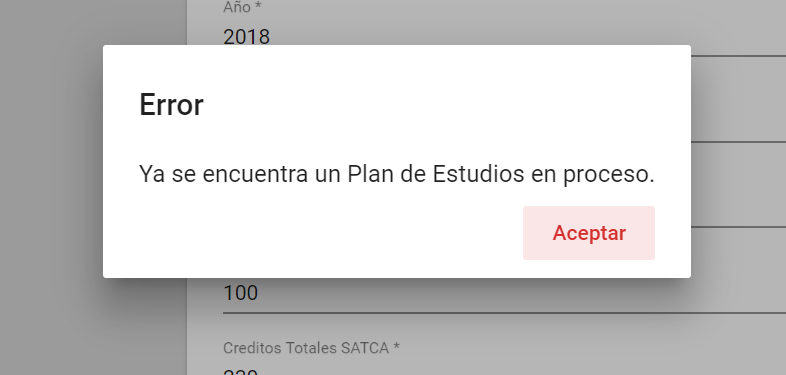
\includegraphics[width=0.7\linewidth]{images/SP4-GPE/error1}}
		\caption{Plan de Estudio en proceso}
		\label{error1}
	\end{figure}
	
	
	Significa que ya hay un Plan de Estudio en proceso. Al dar clic en en botón \IUbutton{Aceptar}, el sistema redirecciona al Jefe de Departamento de Desarrollo e Innovación Curricular a la pantalla de \hyperlink{registrarPE}{\textit{Registrar Planes de Estudios}}. 
	
	\item Campos vacíos al momento de agregar un nuevo Plan de Estudio
	
	Si el Jefe de Departamento de Desarrollo e Innovación Curricular deja en blanco algún campo del formulario, y posteriormente da clic en el botón \IUbutton{Registrar}, el sistema muestra el siguiente mensaje:
	%Imagen MSG32
		\begin{figure}[!hbtp]
		\centering
		\hypertarget{ms4}{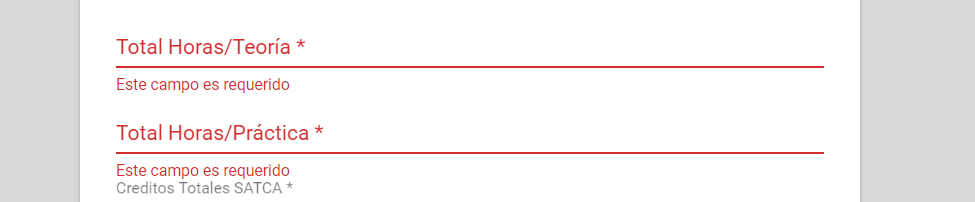
\includegraphics[width=0.7\linewidth]{images/SP4-GPE/m4}}
		\caption{Campos obligatorios}
		\label{ms4}
	    \end{figure}
    
	El usuario debe llenar el o los campos que dejo vacío. Si se continúan dejando campos en blanco y dando clic en el botón \IUbutton{Registrar}, aparecerá nuevamente el mensaje, hasta que todos los campos sean llenados.\\
	
	\newpage
	
	\item Los campos ingresados no son válidos
	
	Si al momento de dar clic en el botón \IUbutton{Registrar} aparece el siguiente mensaje:
	%Imagen MSG20
	\begin{figure}[!hbtp]
		\centering
		\hypertarget{ms5}{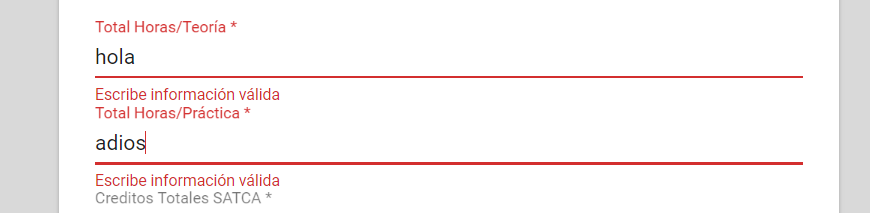
\includegraphics[width=0.7\linewidth]{images/SP4-GPE/m5}}
		\caption{Datos no válidos}
		\label{ms5}
	\end{figure}

	Significa que la composición de los datos ingresados en el formulario no es la correcta, verifíquelos e intente de nuevo.
	
\end{itemize}








